\documentclass{article}
\usepackage[T1]{fontenc}  
\usepackage[utf8]{inputenc}  
\usepackage[vietnamese]{babel}  
\usepackage{graphicx}  
\usepackage{hyperref}
\usepackage[utf8]{vietnam}
\usepackage{amsmath}
\usepackage{enumitem}
\usepackage{tikz}
\usepackage{tabularx}
\usepackage{makecell}
\usepackage[table]{xcolor}
\usepackage[a4paper, left=1.5in, right=1in, top=1in, bottom=1in]{geometry} % Điều chỉnh lề
\usepackage{setspace} % Để điều chỉnh giãn dòng
\usepackage{indentfirst} % Thụt lề đầu dòng
\usepackage{amsmath,amsfonts,amssymb}
\usepackage{geometry}
\geometry{top=2.5cm,bottom=2.5cm,left=3cm,right=2cm}
\usepackage{setspace}
\onehalfspacing
\usepackage{times}
\usepackage{sectsty}
\sectionfont{\large\bfseries}
\subsectionfont{\normalsize\bfseries}
\usepackage{tocloft}
\usepackage{parskip}
\setlength{\parskip}{0.5em}
\usepackage{noto}
% \usepackage[fontsize=13pt]{scrextend} 

\usepackage{float}
\usepackage{titlesec}


% Định dạng đoạn văn
\setlength{\parindent}{1.27cm} % Thụt lề đầu dòng 1.27cm
\setlength{\parskip}{6pt} % Khoảng cách giữa các đoạn
\onehalfspacing % Giãn dòng 1.5

\titleformat{\section}
  {\Large\bfseries}{\thesection}{1em}{}

\titleformat{\subsection}
  {\large\bfseries}{\thesubsection}{1em}{}

\titleformat{\subsubsection}
  {\normalsize\bfseries}{\thesubsubsection}{1em}{}

\begin{document}

\begin{titlepage}
    \begin{tikzpicture}[remember picture, overlay]
        % Vẽ khung trang trí gần mép trang
        \draw[thick, rounded corners, draw=blue!50!black] 
            ([shift={(1cm,-1cm)}]current page.north west) 
            rectangle 
            ([shift={(-1cm,1cm)}]current page.south east);
        % Vẽ khung bên trong (tùy chọn)
        \draw[dashed, draw=red!70!black] 
            ([shift={(1.5cm,-1.5cm)}]current page.north west) 
            rectangle 
            ([shift={(-1.5cm,1.5cm)}]current page.south east);
    \end{tikzpicture}

    \vspace*{-1cm} 
    \centering

    % Phần tiêu đề
    {\LARGE \textbf{UỶ BAN NHÂN DÂN THÀNH PHỐ HỒ CHÍ MINH}} \\[0.5cm] % Tạo khoảng cách giữa dòng đầu và dòng sau
    {\Large \textbf{\underline{TRƯỜNG ĐẠI HỌC SÀI GÒN}}} \\[1cm]

    % Chèn logo
    
\includegraphics[width=4cm]{./img/logo.png} \\[1cm]

    % Tiêu đề luận văn
    {\huge \textbf{NHẬN DIỆN BIỂU CẢM KHUÔN MẶT TRONG ĐIỀU KIỆN ÁNH SÁNG YẾU SỬ DỤNG CNN NHẸ KẾT HỢP KỸ THUẬT TĂNG CƯỜNG DỮ LIỆU THÍCH ỨNG}} \\[1.5cm]

    % Mô tả luận văn
    {\Large \textbf{LUẬN VĂN MÔN HỌC NCKH TRONG CNTT}} \\[0.5cm]
    {\Large NGÀNH: CÔNG NGHỆ THÔNG TIN} \\[1cm]

    % Thông tin nhóm sinh viên
    \textbf{Nhóm sinh viên thực hiện: (Nhóm 17)} \\[0.5cm]
    \begin{tabular}{l l}
        \textbf{Họ và tên} & \textbf{MSSV} \\ 
        Văn Tuấn Kiệt & 3122410202 \\ 
        Mai Phúc Lâm & 3122410207 \\ 
        Nguyễn Đức Duy Lâm & 3122410208 \\ 
        Nguyễn Hữu Lộc & 3122410213 \\ 
    \end{tabular}
    \\[1cm]  % Thêm khoảng cách giữa bảng và phần tiếp theo
    % Thông tin giáo viên hướng dẫn
    \textbf{Giáo viên hướng dẫn:} Đỗ Như Tài \\[0.5cm]
    % Ngày tháng
    \textbf{ 05/2025, TP.HCM }
\end{titlepage}

\newpage 
% Áp dụng cỡ chữ 13pt
\begingroup
\fontsize{13pt}{18pt}\selectfont

\begin{center}
    {\LARGE \textbf{BÁO CÁO LUẬN VĂN}} \\[1cm]
\end{center}

\section{Tổng quan vấn đề} % Section 1
\subsection{Lý do chọn đề tài}
Nhận diện biểu cảm khuôn mặt (Facial Expression Recognition - FER) đóng vai trò quan trọng trong các ứng dụng thực tiễn như giao tiếp người-máy, giám sát an ninh, và phân tích hành vi. Tuy nhiên, trong các điều kiện ánh sáng yếu, chẳng hạn như môi trường ban đêm hoặc khu vực thiếu sáng, hiệu quả của các hệ thống FER giảm đáng kể do chất lượng hình ảnh thấp. Các nghiên cứu gần đây (2020--2025) chủ yếu tập trung vào điều kiện ánh sáng lý tưởng, trong khi các giải pháp cho ánh sáng yếu thường phức tạp, đòi hỏi tài nguyên tính toán lớn hoặc không tối ưu cho các thiết bị nhúng. 

Việc phát triển một phương pháp nhận diện biểu cảm hiệu quả trong điều kiện ánh sáng yếu, sử dụng mô hình CNN nhẹ (như MobileNetV3) và kỹ thuật tăng cường dữ liệu thích ứng, không chỉ đáp ứng nhu cầu thực tiễn mà còn mang lại giá trị khoa học thông qua việc cải tiến các kỹ thuật hiện có. Đề tài này được chọn vì tính khả thi trong thời gian nghiên cứu (6 tuần), tính mới trong việc kết hợp các phương pháp đơn giản nhưng hiệu quả, và tiềm năng ứng dụng trong các hệ thống thực tế như camera giám sát hoặc thiết bị IoT.

% Subsection: Vấn đề nghiên cứu
\subsection{Vấn đề nghiên cứu}
Trong điều kiện ánh sáng yếu, các mô hình nhận diện biểu cảm khuôn mặt truyền thống thường gặp khó khăn do độ tương phản thấp, nhiễu ảnh, và mất chi tiết khuôn mặt. Các phương pháp hiện tại như sử dụng GAN (Generative Adversarial Networks) hoặc Retinex-based preprocessing tuy hiệu quả nhưng phức tạp, yêu cầu thời gian huấn luyện lâu và tài nguyên tính toán lớn, không phù hợp với các ứng dụng thời gian thực hoặc thiết bị có tài nguyên hạn chế. Ngoài ra, các kỹ thuật tăng cường dữ liệu cố định (fixed augmentation) không tối ưu vì không thích nghi với mức độ ánh sáng yếu khác nhau của từng ảnh.

Vấn đề nghiên cứu được đặt ra là: Làm thế nào để phát triển một hệ thống nhận diện biểu cảm khuôn mặt trong điều kiện ánh sáng yếu, sử dụng mô hình CNN nhẹ và kỹ thuật tăng cường dữ liệu thích ứng, nhằm đạt được độ chính xác cao, tốc độ xử lý nhanh, và khả năng triển khai trên các thiết bị nhúng?

% Subsection: Mục tiêu nghiên cứu
\subsection{Mục tiêu nghiên cứu}
Mục tiêu tổng quát của nghiên cứu là xây dựng một hệ thống nhận diện biểu cảm khuôn mặt hiệu quả trong điều kiện ánh sáng yếu, sử dụng mạng nơ-ron tích chập nhẹ (MobileNetV3) kết hợp với kỹ thuật tăng cường dữ liệu thích ứng. Các mục tiêu cụ thể bao gồm:
\begin{enumerate}
    \item Phát triển một pipeline tăng cường dữ liệu thích ứng, tự động điều chỉnh các kỹ thuật tăng cường dựa trên mức độ ánh sáng yếu của từng ảnh.
    \item Huấn luyện và tinh chỉnh mô hình MobileNetV3 để nhận diện biểu cảm khuôn mặt trong điều kiện ánh sáng yếu với độ chính xác cao.
    \item Đánh giá và so sánh hiệu quả của phương pháp đề xuất với các kỹ thuật tăng cường dữ liệu cố định và các mô hình CNN khác (nếu khả thi).
\end{enumerate}

% Subsection: Câu hỏi nghiên cứu
\subsection{Câu hỏi nghiên cứu}
Nghiên cứu tập trung trả lời các câu hỏi sau:
\begin{enumerate}
    \item Làm thế nào để thiết kế một pipeline tăng cường dữ liệu thích ứng, hiệu quả trong việc cải thiện chất lượng ảnh ánh sáng yếu cho nhận diện biểu cảm khuôn mặt?
    \item Mô hình MobileNetV3 có thể đạt được độ chính xác tương đương hoặc vượt trội so với các kỹ thuật tăng cường dữ liệu cố định trong điều kiện ánh sáng yếu không?
    \item Các kỹ thuật tăng cường dữ liệu thích ứng ảnh hưởng như thế nào đến hiệu suất của mô hình CNN nhẹ trong nhận diện biểu cảm khuôn mặt?
\end{enumerate}

% Subsection: Phạm vi nghiên cứu
\subsection{Phạm vi nghiên cứu}
\begin{itemize}
    \item \textbf{Đối tượng nghiên cứu}: Các biểu cảm khuôn mặt (ví dụ: vui, buồn, tức giận, ngạc nhiên) trong điều kiện ánh sáng yếu, được mô phỏng hoặc thu thập từ bộ dữ liệu công khai FER-2013.
    \item \textbf{Phạm vi không gian}: Nghiên cứu tập trung vào xử lý hình ảnh tĩnh (static images), không bao gồm dữ liệu video hoặc dữ liệu đa phổ.
    \item \textbf{Phạm vi thời gian}: Nghiên cứu được thực hiện trong 8 tuần, từ tháng 4 đến tháng 5 năm 2025, với các thí nghiệm dựa trên dữ liệu công khai và mô hình pre-trained.
    \item \textbf{Phạm vi kỹ thuật}: Sử dụng mô hình CNN nhẹ (MobileNetV3) và các kỹ thuật tăng cường dữ liệu như gamma correction, histogram equalization, được triển khai bằng Python với các thư viện TensorFlow/Keras và OpenCV.
\end{itemize}

\section{Lược khảo tài liệu} % Section 2
\subsection{Tổng hợp các tài liệu, nghiên cứu trước liên quan}

\subsubsection{Nghiên cứu về nhận diện biểu cảm khuôn mặt (FER)}
Nhận diện biểu cảm khuôn mặt (Facial Expression Recognition - FER) là một lĩnh vực trọng điểm trong thị giác máy tính. Từ đầu những năm 2000, các phương pháp truyền thống như LBP, HOG, hoặc SIFT kết hợp với SVM từng chiếm ưu thế. Tuy nhiên, chúng không hiệu quả trong điều kiện ánh sáng thay đổi hoặc góc nhìn khác nhau. Từ năm 2014, học sâu – đặc biệt là CNN – đã nâng cao độ chính xác mô hình FER. Các kiến trúc như VGGNet, ResNet, InceptionNet đạt độ chính xác 70--75\% trên FER-2013 nhưng yêu cầu tài nguyên tính toán lớn \cite{goodfellow2013challenges}.

\subsubsection{Ảnh hưởng của điều kiện ánh sáng yếu}
Zhang et al. (2019), Wang et al. (2022) đã chứng minh rằng ảnh thiếu sáng làm giảm hiệu quả của mô hình FER. Các phương pháp dựa trên GAN như EnlightenGAN hoặc RetinexNet giúp cải thiện nhưng đòi hỏi GPU mạnh, không phù hợp với thiết bị thực tế như điện thoại hoặc camera nhúng \cite{zhang2019ganfer, wang2022lowlight}.

\subsubsection{Các kỹ thuật tiền xử lý ảnh tăng cường sáng}
\textbf{Gamma Correction}: điều chỉnh độ sáng theo hàm \(I_{out} = I_{in}^\gamma\). Với \(\gamma < 1\), ảnh được làm sáng \cite{ying2017gamma}.\par
\textbf{CLAHE}: nâng cao độ tương phản cục bộ, phù hợp ảnh có vùng sáng tối không đều, đã được sử dụng hiệu quả trong FER \cite{pizer1987clahe}.

\subsubsection{Mô hình học sâu nhẹ: MobileNetV3}
MobileNetV3 (Howard et al., 2019) là CNN nhẹ, tối ưu cho thiết bị di động, gồm kỹ thuật như depthwise separable convolution, squeeze-and-excitation và NAS. MobileNetV3-Small có khoảng 2.5 triệu tham số, cân bằng tốt giữa độ chính xác và hiệu suất, tuy nhiên chưa được nghiên cứu sâu trong FER dưới điều kiện ánh sáng yếu \cite{howard2019mobilenetv3, sandler2018mobilenetv2}.

\begin{figure}[H]
    \centering
    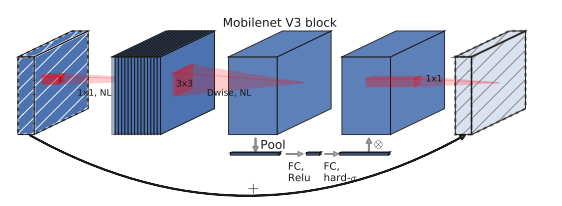
\includegraphics[width=0.7\textwidth]{img/mobinetv3.png} % Đường dẫn tương đối
    \caption{Mô hình MobileNetV3.}
    \label{fig:emotion_distribution11}
\end{figure}

Hình \ref{fig:emotion_distribution11} giải thích cấu trúc một khối MobileNetV3, được xây dựng dựa trên kiến trúc Inverted Residual Block của MobileNetV2, nhưng có thêm mô-đun Squeeze-and-Excitation (SE) để nâng cao độ chính xác. Trong khối này, nhánh chính gồm ba lớp: 1×1 convolution (Expansion), 3×3 depthwise convolution, và 1×1 convolution (Projection). Nhánh phụ SE được chèn vào giữa, gồm Global Average Pooling, hai lớp fully connected (FC → ReLU → FC → Hard-Sigmoid), rồi nhân với đầu vào để thực hiện điều chỉnh trọng số theo ngữ cảnh toàn cục. Kiến trúc này giúp mô hình nhẹ, nhanh và hiệu quả hơn trong việc trích xuất đặc trưng, đặc biệt phù hợp với thiết bị di động hoặc nhúng \cite{howard2019mobilenetv3}.

\subsection{Cơ sở lý thuyết của nghiên cứu}
Nghiên cứu kết hợp tiền xử lý ảnh thích ứng theo điều kiện ánh sáng và mô hình CNN nhẹ – MobileNetV3 để tăng hiệu suất FER trong điều kiện ánh sáng yếu.

\subsubsection{Tiền xử lý ảnh trong điều kiện ánh sáng yếu}
\textbf{Gamma Correction} \cite{ying2017gamma}: hàm phi tuyến giúp làm sáng ảnh thiếu sáng. Ying et al. (2017) chỉ ra rằng \(\gamma\) phù hợp có thể nâng cao chất lượng ảnh mà không gây nhiễu.\par
\textbf{CLAHE} \cite{pizer1987clahe}: phân tích cục bộ từng vùng ảnh, cải thiện chi tiết biểu cảm ở vùng mắt, miệng.\par
\textbf{Tính thích ứng} \cite{wang2022lowlight}: thuật toán tự động phân tích histogram và độ sáng trung bình để chọn phương pháp phù hợp.

\subsubsection{Nhận diện biểu cảm bằng mô hình CNN nhẹ – MobileNetV3}
MobileNetV3-Small \cite{howard2019mobilenetv3}: có khoảng 2.5 triệu tham số, thích hợp cho thiết bị nhúng. Nghiên cứu dùng mô hình này để fine-tune phân loại 7 biểu cảm.\par
\textbf{Kỹ thuật chính}: Depthwise Separable Convolution \cite{howard2017mobilenets}, SE Module \cite{hu2018squeeze}, Hard-Swish Activation.

\subsubsection{Pipeline đề xuất trong nghiên cứu}
Dựa trên hai thành phần lý thuyết đã trình bày, nghiên cứu đề xuất pipeline xử lý gồm 3 giai đoạn chính như trong Bảng~\ref{tab:pipeline}.

\begin{table}[H]
\centering
\caption{Pipeline đề xuất trong nghiên cứu}
\label{tab:pipeline}
\begin{tabular}{|p{4cm}|p{10cm}|}
\hline
\textbf{Giai đoạn} & \textbf{Nội dung} \\
\hline
\textbf{Tiền xử lý ảnh} &
\begin{itemize}[leftmargin=*]
    \item Chuyển ảnh sang ảnh grayscale.
    \item Tính độ sáng trung bình $\mu$.
    \item Nếu $\mu < T_1$: áp dụng gamma correction với $\gamma = 0.5$.
    \item Nếu $T_1 < \mu < T_2$: áp dụng gamma correction với $\gamma = 0.8$.
    \item Nếu $\mu > T_2$: áp dụng contrast stretching nhẹ.
\end{itemize} \\
\hline
\textbf{Học biểu cảm} &
\begin{itemize}[leftmargin=*]
    \item Ảnh sau tiền xử lý được đưa vào mô hình MobileNetV3-Small.
    \item Mô hình được fine-tune để phân loại 7 biểu cảm: vui, buồn, giận, sợ, bất ngờ, ghê tởm, trung tính.
\end{itemize} \\
\hline
\textbf{Đánh giá mô hình} &
\begin{itemize}[leftmargin=*]
    \item Thực hiện trên tập test có và không áp dụng tăng cường ảnh.
    \item Sử dụng các chỉ số đánh giá:
    \begin{itemize}
        \item Accuracy
        \item F1-score
        \item Time
        \item Size
        \item Confusion Matrix
    \end{itemize}
    \item So sánh với baseline không áp dụng tăng cường để đánh giá hiệu quả thực sự.
\end{itemize} \\
\hline
\end{tabular}
\end{table}

Bảng~\ref{tab:pipeline} mô tả chi tiết \textbf{pipeline xử lý} được đề xuất trong nghiên cứu, bao gồm ba giai đoạn chính: \textit{tiền xử lý ảnh}, \textit{học biểu cảm}, và \textit{đánh giá mô hình}. Trong giai đoạn tiền xử lý, ảnh đầu vào được chuyển sang ảnh xám và điều chỉnh độ sáng hoặc tương phản dựa trên giá trị trung bình $\mu$ của ảnh. Tùy theo mức độ sáng, các kỹ thuật như gamma correction, contrast stretching sẽ được áp dụng nhằm cải thiện chất lượng ảnh đầu vào.

Tiếp theo, giai đoạn học biểu cảm sử dụng mô hình \textit{MobileNetV3-Small} đã được tinh chỉnh (fine-tune) để phân loại bảy loại biểu cảm khuôn mặt phổ biến: vui, buồn, giận, sợ, bất ngờ, ghê tởm và trung tính.

Cuối cùng, mô hình được đánh giá trên tập kiểm thử với và không có áp dụng kỹ thuật tăng cường ảnh. Các chỉ số đánh giá bao gồm Accuracy, Precision, Recall, F1-score và ma trận nhầm lẫn (Confusion Matrix). Kết quả mô hình sẽ được so sánh với một mô hình baseline không áp dụng tăng cường ảnh nhằm đánh giá hiệu quả thực sự của pipeline đề xuất.


\begin{figure}[H]
    \centering
    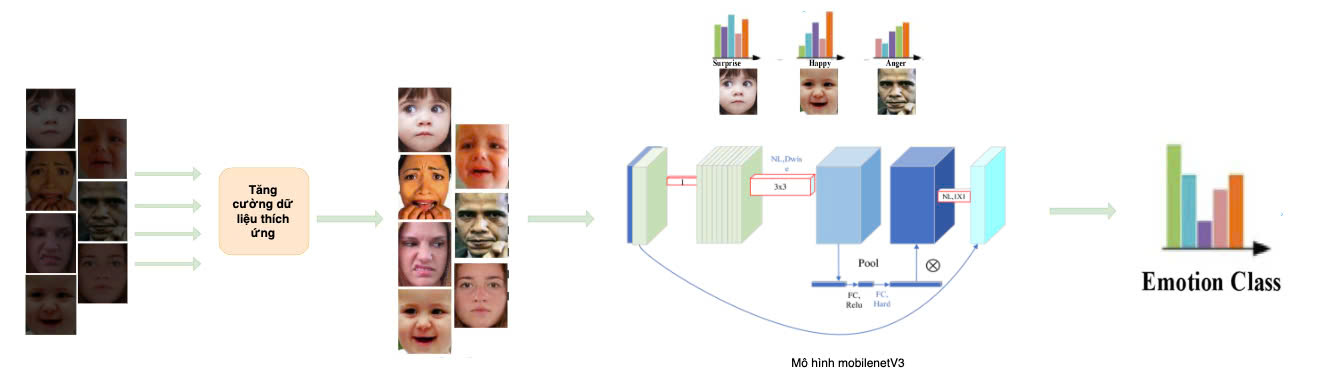
\includegraphics[width=0.9\textwidth]{img/pineline.jpg} % Đường dẫn tương đối
    \caption{Pipeline đề xuất}
    \label{fig:pineline}
\end{figure}

Hình~\ref{fig:pineline} cho thấy pipeline đề xuất cho hệ thống nhận diện cảm xúc khuôn mặt. Dữ liệu ảnh đầu vào được tăng cường bằng cách điều chỉnh độ sáng nhằm cải thiện khả năng nhận diện trong các điều kiện ánh sáng khác nhau. Sau đó, ảnh được đưa vào mô hình MobileNetV3 để trích xuất đặc trưng và phân loại cảm xúc đầu ra.

\subsection{Phân tích điểm mạnh, điểm yếu của các nghiên cứu trước và hướng kế thừa}

\subsubsection{Điểm mạnh}
\begin{itemize}
    \item Các mô hình học sâu, như CNN, cải thiện đáng kể độ chính xác nhận diện biểu cảm khuôn mặt (FER), đạt trên 70\% trên tập FER-2013 \cite{mollahosseini2016}.
    \item MobileNetV3 có hiệu suất cao, kích thước nhỏ (dưới 5MB) và tiết kiệm tài nguyên, phù hợp cho thiết bị nhúng \cite{howard2019, sandler2018}.
    \item Kỹ thuật tăng cường độ sáng hiệu quả, dễ triển khai và ít tốn tài nguyên tính toán.
\end{itemize}

\subsubsection{Hạn chế}
\begin{itemize}
    \item Các nghiên cứu FER trước đây ít tập trung vào điều kiện ánh sáng yếu, dẫn đến giảm độ chính xác 20--30\% trong môi trường thực tế \cite{mollahosseini2016}.
    \item Thiếu các phương pháp tiền xử lý thích ứng, khiến mô hình kém hiệu quả khi xử lý ảnh có độ sáng không đồng đều \cite{zhang2019, wang2020}.
    \item Các kỹ thuật tăng sáng dựa trên GAN, như EnlightenGAN và RetinexNet, yêu cầu tài nguyên lớn (hàng GB bộ nhớ GPU), không khả thi cho thiết bị hạn chế \ listes \cite{zhang2019}.
\end{itemize}

\subsubsection{Hướng kế thừa và phát triển}
\begin{itemize}
    \item Chọn MobileNetV3-Small làm backbone.
    \item Thiết kế pipeline có bước xử lý ảnh thích ứng đầu vào.
    \item Mô phỏng tập FER-2013 thiếu sáng để kiểm thử.
    \item Ưu tiên tăng sáng đơn giản thay vì GAN.
\end{itemize}

% Chương 2.4 - Cơ sở lý thuyết của thuật toán tăng cường dữ liệu thích ứng
\subsection{Cơ sở lý thuyết của thuật toán tăng cường dữ liệu thích ứng} % 2.4

\subsubsection{Lý do phát triển thuật toán} % 2.4.1
Trong bài toán nhận diện biểu cảm khuôn mặt (FER -- Facial Expression Recognition) dưới điều kiện ánh sáng yếu, hình ảnh khuôn mặt thường bị suy giảm chất lượng nghiêm trọng do hiện tượng thiếu sáng toàn cục hoặc cục bộ. Điều này dẫn đến hiện tượng mất chi tiết, đặc biệt ở các vùng chứa đặc trưng biểu cảm quan trọng như mắt, miệng, nếp nhăn. Kết quả là mô hình học sâu, vốn phụ thuộc vào độ tương phản và cấu trúc cục bộ, sẽ khó khăn trong việc nhận dạng chính xác. 

Các kỹ thuật tăng cường dữ liệu truyền thống như histogram equalization hoặc gamma correction thường được áp dụng đồng loạt cho toàn bộ dữ liệu huấn luyện. Tuy nhiên, cách tiếp cận này bỏ qua tính biến thiên về mức sáng của từng ảnh đầu vào. Cụ thể:
\begin{itemize}[]
    \item Với ảnh quá tối, tăng sáng quá mức dễ làm mất chi tiết do bão hòa điểm ảnh.
    \item Với ảnh sáng vừa đủ, tăng cường không cần thiết có thể làm biến dạng đặc trưng tự nhiên, dẫn đến suy giảm hiệu quả học.
\end{itemize}

Do đó, nghiên cứu này đề xuất một thuật toán tăng cường dữ liệu thích ứng, có khả năng phân tích đặc trưng ánh sáng riêng của từng ảnh, từ đó lựa chọn kỹ thuật xử lý phù hợp, đơn giản nhưng hiệu quả và phù hợp để huấn luyện với mô hình nhẹ như MobileNetV3-Small.

\subsubsection{Các thành phần lý thuyết chính} % 2.4.2
\subsubsection*{(a) Phân tích độ sáng của ảnh}

Để xác định ảnh đầu vào có cần tăng cường hay không, và nếu cần thì sử dụng phương pháp nào, cần phân tích một số đặc trưng cơ bản về độ sáng:


\begin{itemize}[]
    \item \textbf{Độ sáng trung bình (mean intensity)}: Được tính trên ảnh chuyển sang thang xám (grayscale) hoặc kênh Y (luminance) trong không gian YUV.
    
    \[ \mu = \frac{1}{H \times W} \sum_{i=1}^{H} \sum_{j=1}^{W} I(i,j) \]
    
    \item \textbf{Độ lệch chuẩn (standard deviation)}: Đánh giá mức độ phân tán sáng tối, cho biết ảnh có sáng đồng đều hay có vùng sáng -- vùng tối xen kẽ.
    \item \textbf{Histogram phân bố pixel}: Dùng để xác định ảnh có độ tương phản thấp (hẹp histogram) hoặc bị lệch về vùng tối.
\end{itemize}

\subsubsection*{(b) Các kỹ thuật tăng cường ánh sáng được sử dụng}
\begin{itemize}[]
    \item \textbf{Gamma Correction:}
    \[ I_{\text{out}} = I_{\text{in}}^{\gamma} \]
    \begin{itemize}[]
        \item $\gamma < 1$: ảnh được làm sáng lên.
        \item $\gamma > 1$: ảnh bị làm tối hơn.
    \end{itemize}
    Việc chọn giá trị $\gamma$ được tính toán dựa trên giá trị độ sáng trung bình $\mu$ của ảnh.

    \item \textbf{Histogram Equalization (HE)}:
    Phân bố lại giá trị pixel để làm tăng độ tương phản tổng thể. Phù hợp khi histogram bị tập trung ở vùng tối (low dynamic range). Tuy nhiên, dễ gây nhiễu ở ảnh có noise.

    \item \textbf{Contrast Stretching:}
    Kéo dãn mức độ sáng từ dải cường độ cũ về dải chuẩn 0--255:
    \[ I_{\text{out}} = \frac{I_{\text{in}} - I_{\min}}{I_{\max} - I_{\min}} \times 255 \]
    

      \begin{figure}[H]
    \centering
    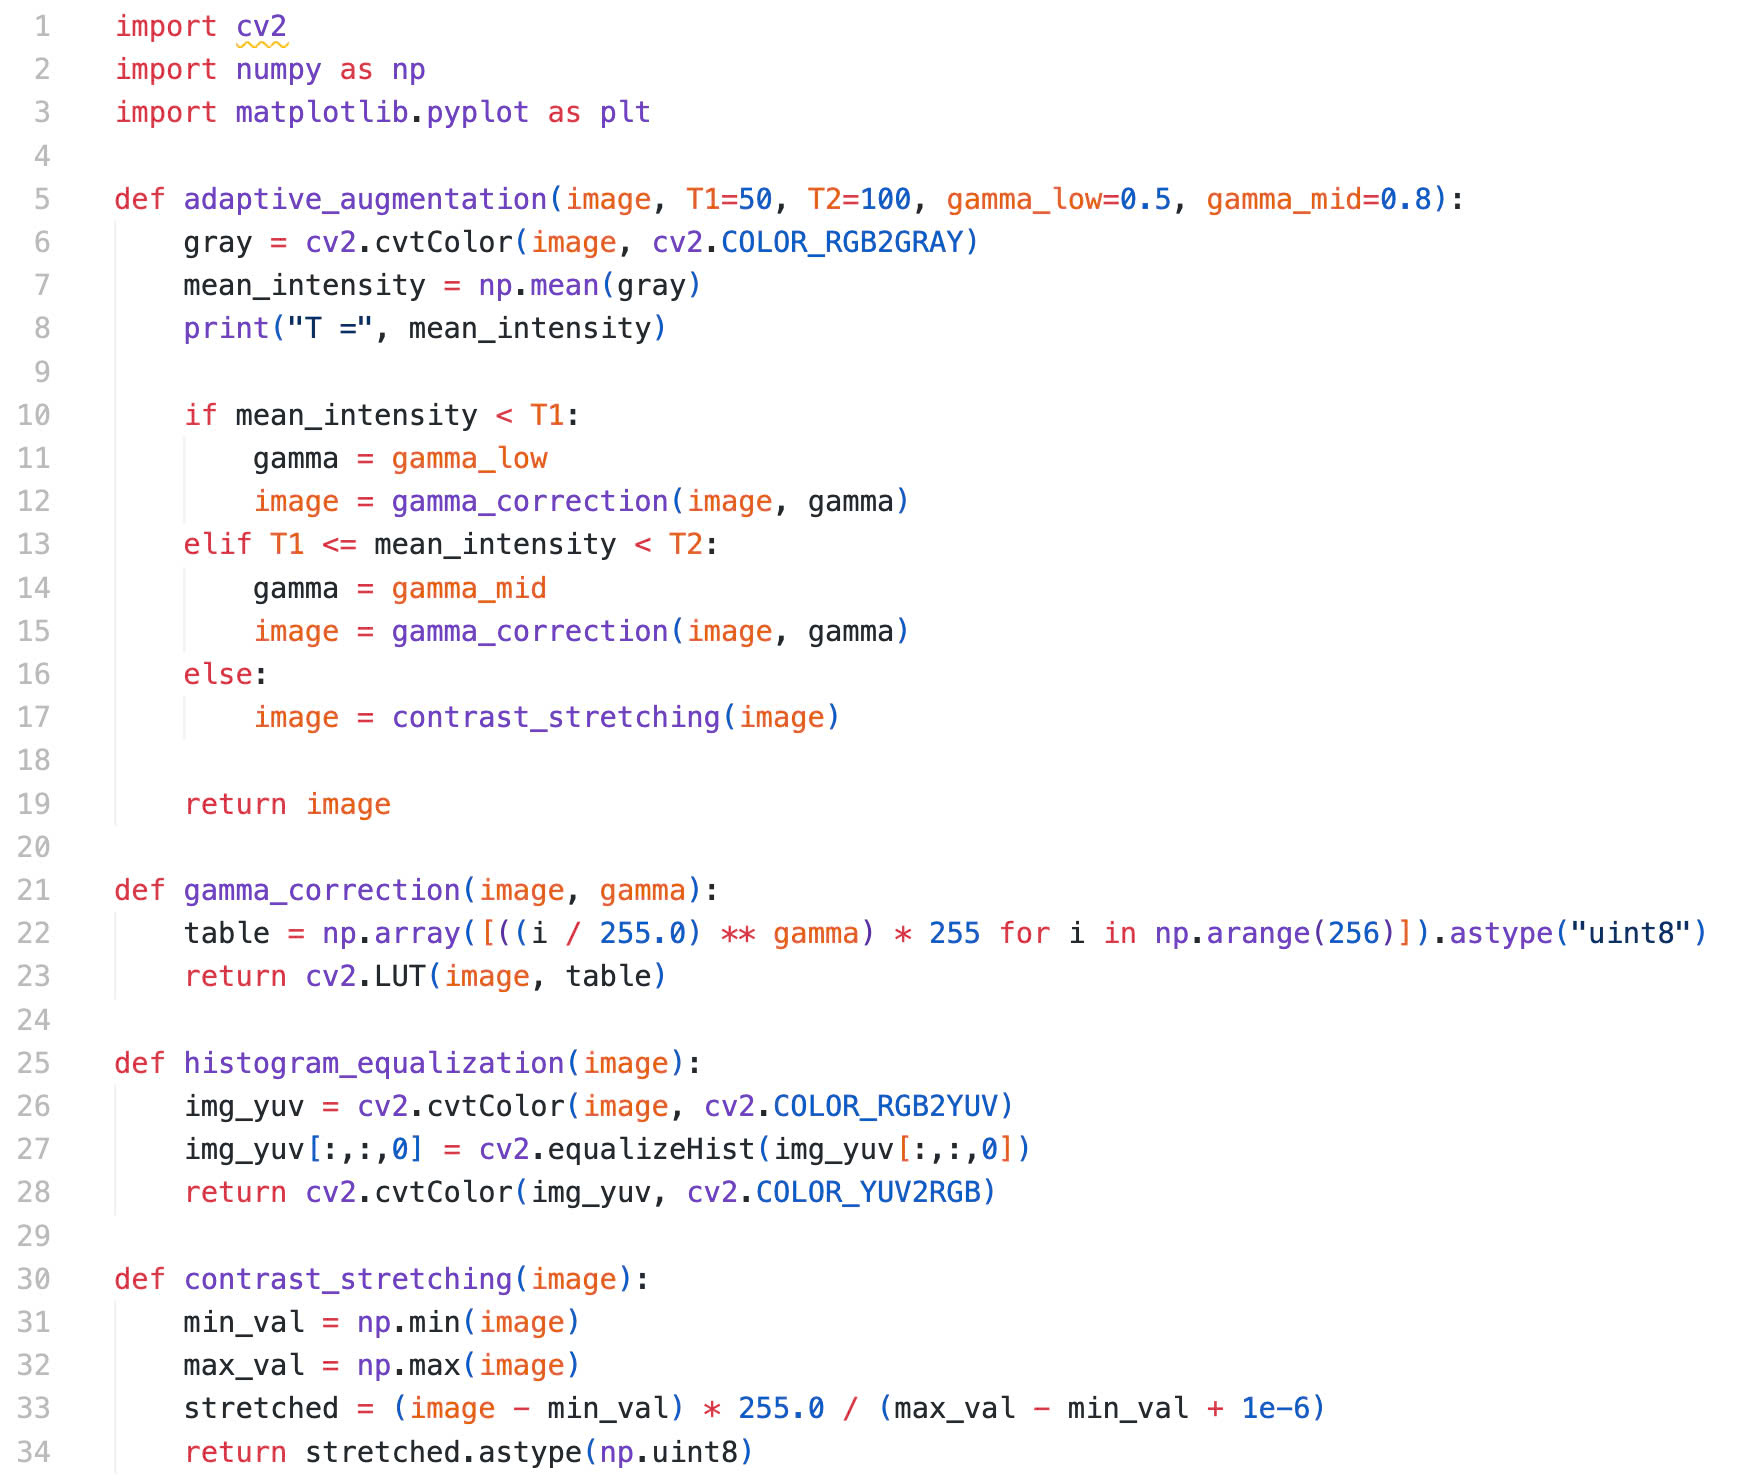
\includegraphics[width=0.7\textwidth]{img/thuatToan_01.jpg} % Đường dẫn tương đối
    \label{fig:emotion_distribution}
\end{figure}
  \begin{figure}[H]
    \centering
    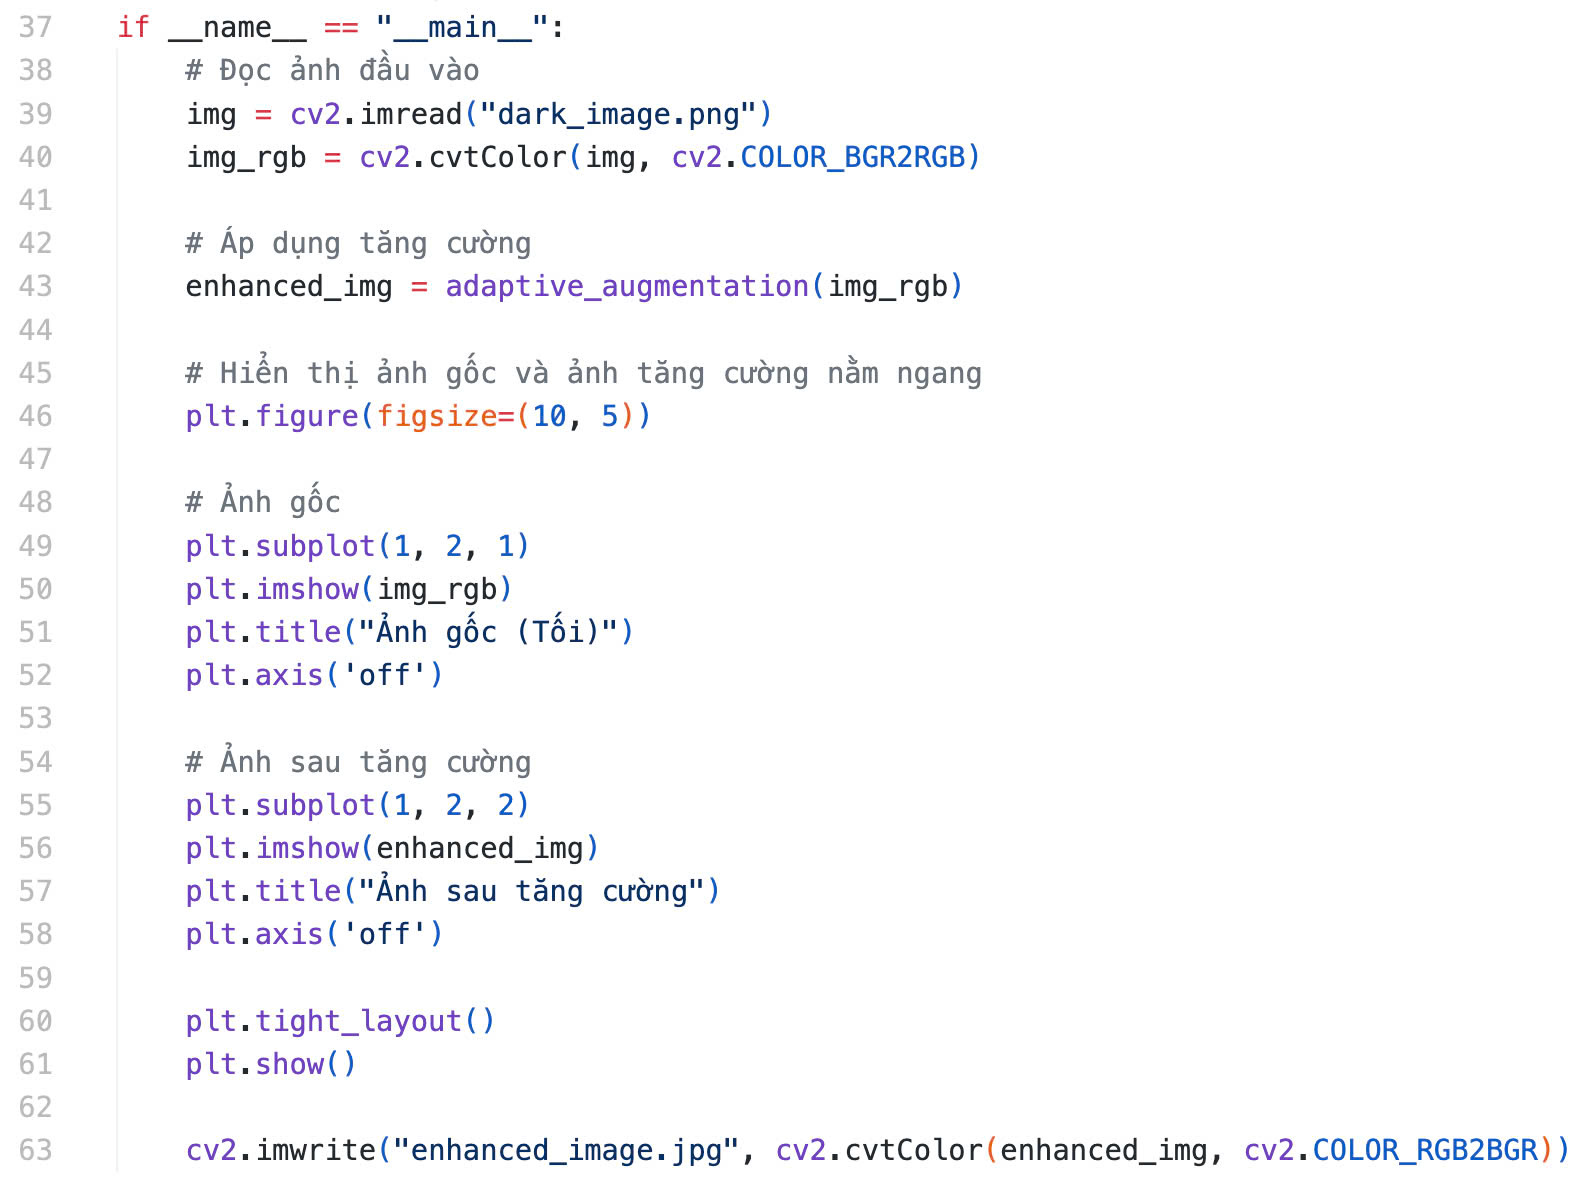
\includegraphics[width=0.7\textwidth]{img/thuatToan_02.jpg} % Đường dẫn tương đối
    \caption{Code minh họa}
    \label{fig:emotion_distribution}
\end{figure}



   
\end{itemize}

    
Đoạn code trên làm nhiệm vụ tăng cường ảnh thích ứng dựa theo độ sáng trung bình của ảnh đầu vào. Cụ thể, ảnh đầu vào sẽ được chuyển sang thang xám để tính giá trị cường độ sáng trung bình (mean intensity). Dựa vào ngưỡng định sẵn T1 và T2, ảnh sẽ được xử lý theo ba trường hợp:
\begin{itemize}[]
     \item Nếu ảnh quá tối ($\mu < T1$): áp dụng gamma correction với hệ số gamma thấp.
     \item Nếu ảnh hơi tối (T1 <= $\mu < T2$): dùng gamma correction với hệ số trung bình.
     \item Nếu ảnh đủ sáng ($\mu >= T2$): dùng contrast stretching để cải thiện độ tương phản.
\end{itemize}
    
Ảnh sau khi tăng cường sẽ được hiển thị song song với ảnh gốc và lưu ra tệp tin mới.


 \begin{figure}[H]
    \centering
    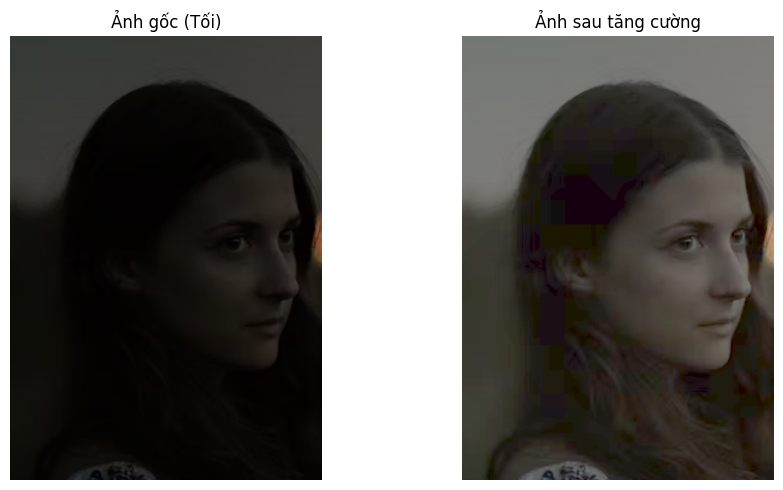
\includegraphics[width=0.7\textwidth]{img/anhsautangcuong.png} % Đường dẫn tương đối
    \caption{Ảnh trước và sau khi tăng cường}
    \label{fig:emotion_distribution22}
\end{figure}

Hình~\ref{fig:emotion_distribution22} thể hiện kết quả xử lý ảnh tối bằng phương pháp Gamma Correction. Ảnh bên trái là ảnh gốc trong điều kiện ánh sáng yếu, với nhiều chi tiết khuôn mặt bị chìm trong vùng tối, gây khó khăn cho việc nhận diện. Sau khi áp dụng Gamma Correction (ảnh bên phải), độ sáng tổng thể được cải thiện đáng kể, các đặc trưng như mắt, tóc và đường nét khuôn mặt trở nên rõ ràng hơn. Phương pháp này giúp ảnh trở nên dễ phân tích hơn đối với các mô hình học sâu, đặc biệt trong bài toán nhận diện biểu cảm dưới điều kiện ánh sáng yếu.


\subsubsection*{(c) Tính thích ứng của thuật toán}
Thuật toán sẽ:
\begin{itemize}[]
    \item Tính toán độ sáng trung bình ($\mu$) và độ lệch chuẩn ($\sigma$) của từng ảnh đầu vào.
    \item Dựa vào hai ngưỡng xác định trước $T_1$ và $T_2$, phân loại mức độ ánh sáng:
    \begin{itemize}[]
        \item $\mu < T_1$ (ảnh rất tối): áp dụng gamma nhỏ (0.3--0.5).
        \item $T_1 \le \mu < T_2$ (tối vừa): áp dụng gamma nhẹ (0.7--0.9) hoặc HE.
        \item $\mu \ge T_2$ (sáng đủ): không tăng cường hoặc chỉ contrast stretching nhẹ.
    \end{itemize}
\end{itemize}
Cách tiếp cận này giúp mỗi ảnh được tăng cường đúng mức, tránh làm hỏng đặc trưng gốc hoặc gây dư sáng.

\subsubsection{Nguồn cảm hứng và các nghiên cứu liên quan} % 2.4.3

Retinex-based methods (Zhang et al., 2022) đề xuất kỹ thuật phân tách ảnh thành hai thành phần: phản xạ và ánh sáng chiếu vào, sau đó tái cấu trúc lại ảnh với độ sáng cải thiện. Phương pháp này cho kết quả nâng cao rõ rệt nhưng đòi hỏi thuật toán phức tạp và tài nguyên tính toán lớn, do đó khó triển khai trên các thiết bị nhúng.

GAN-based methods như EnlightenGAN (Zhang et al., 2022) sử dụng mạng sinh ảnh để tạo lại phiên bản ảnh có ánh sáng tốt hơn từ ảnh thiếu sáng ban đầu. Mặc dù đem lại chất lượng thị giác cao, nhưng các mô hình GAN thường yêu cầu GPU mạnh và thời gian xử lý lâu, khiến chúng không phù hợp với các ứng dụng thời gian thực trên thiết bị di động.

Trong khi đó, các nghiên cứu như (Ying et al. 2017) cho thấy các phương pháp tăng cường đơn giản như Gamma Correction, Contrast Stretching nếu được lựa chọn phù hợp theo đặc trưng đầu vào, vẫn mang lại hiệu quả đáng kể. Điều này truyền cảm hứng cho việc thiết kế thuật toán tăng cường thích ứng trong nghiên cứu này – vốn sử dụng phân tích độ sáng ảnh để lựa chọn kỹ thuật phù hợp, thay vì áp dụng cố định một phương pháp cho mọi trường hợp.

Từ các nghiên cứu trên, thuật toán của nhóm đề xuất kế thừa ý tưởng \textit{adaptive preprocessing}, nhưng được đơn giản hóa để giảm chi phí tính toán và đảm bảo tính linh hoạt, phù hợp với các mô hình nhẹ như MobileNetV3.


\section{Phương pháp nghiên cứu} % section 3

\subsection{Thiết kế nghiên cứu} % section 3.1
Nghiên cứu được thiết kế theo phương pháp định lượng, tập trung vào việc xây dựng và đánh giá hiệu suất của các mô hình học sâu trong bài toán nhận diện biểu cảm khuôn mặt (Facial Expression Recognition - FER) trong điều kiện ánh sáng yếu. Phương pháp định lượng được chọn vì mục tiêu nghiên cứu là đo lường các chỉ số hiệu suất cụ thể (Accuracy, Precision, Recall, F1-score và thời gian suy luận) của hai mô hình CNN: MobileNetV3 (mô hình nhẹ) và ResNet18 (mô hình sâu hơn), khi áp dụng kỹ thuật tăng cường dữ liệu thích ứng.

Quá trình nghiên cứu bao gồm ba giai đoạn chính:
\begin{itemize}
    \item \textbf{Tiền xử lý dữ liệu:} Sử dụng tập dữ liệu FER-2013, áp dụng các kỹ thuật tăng cường dữ liệu thích ứng để mô phỏng điều kiện ánh sáng yếu.
    \item \textbf{Huấn luyện và tối ưu mô hình:} Triển khai MobileNetV3 và ResNet18, tinh chỉnh các tham số để phù hợp với bài toán FER.
    \item \textbf{Đánh giá và so sánh:} So sánh hiệu suất và thời gian suy luận của các mô hình khi có và không áp dụng kỹ thuật tăng cường dữ liệu thích ứng.
\end{itemize}

\subsection{Đối tượng và mẫu nghiên cứu} % section 3.2
\subsubsection{Đối tượng nghiên cứu}
Đối tượng nghiên cứu là các kỹ thuật nhận diện biểu cảm khuôn mặt trong điều kiện ánh sáng yếu, với trọng tâm vào:
\begin{itemize}
    \item \textbf{Mô hình học sâu:} MobileNetV3 và ResNet18 dùng để phân loại 7 biểu cảm khuôn mặt (vui, buồn, tức giận, sợ hãi, ngạc nhiên, ghê tởm, trung lập).
    \item \textbf{Kỹ thuật tăng cường dữ liệu thích ứng:} Các phương pháp như gamma correction, contrast stretching và histogram equalization, được điều chỉnh dựa trên đặc trưng ánh sáng của hình ảnh.
\end{itemize}

\subsubsection{Mẫu nghiên cứu}
Mẫu nghiên cứu là tập dữ liệu FER-2013, chứa 35.887 hình ảnh khuôn mặt (48x48 pixel, ảnh xám) được phân loại thành 7 biểu cảm. Tập dữ liệu được chia như sau:
\begin{itemize}
    \item Tập huấn luyện: 22.968 hình ảnh (~64\%).
    \item Tập xác thực (validation): 5.741 hình ảnh (~16\%).
    \item Tập kiểm tra: 7.178 hình ảnh (~20\%).
\end{itemize}


Nhằm mô phỏng điều kiện ánh sáng yếu, một tập dữ liệu phụ được tạo ra bằng cách giảm độ sáng của ảnh gốc. Quá trình này thực hiện bằng cách chuyển ảnh sang không gian màu HSV, giảm kênh độ sáng (V) theo một hệ số cố định, sau đó chuyển lại về không gian RGB. Cụ thể, độ sáng được giảm xuống 10\% so với ảnh ban đầu.

\subsection{Cách thu thập dữ liệu}
Dữ liệu được thu thập từ tập dữ liệu FER-2013 công khai trên nền tảng Kaggle. Các bước gồm:

\subsubsection*{Thu thập dữ liệu}
\begin{itemize}
    \item Tải tập dữ liệu FER-2013 từ Kaggle.
    \item Kiểm tra tính toàn vẹn (số lượng ảnh, định dạng, chất lượng).
\end{itemize}

\subsubsection*{Tiền xử lý dữ liệu}

Các bước tiền xử lý được thực hiện nhằm cải thiện chất lượng ảnh đầu vào và mô phỏng các điều kiện môi trường khác nhau, cụ thể như sau:

\begin{itemize}
    \item \textbf{Chuẩn hóa hình ảnh}: Loại bỏ nhiễu và đảm bảo định dạng đồng nhất (kích thước ảnh, không gian màu), giúp mô hình huấn luyện ổn định hơn.
    
    \item \textbf{Mô phỏng điều kiện ánh sáng yếu}: Để mô phỏng môi trường có ánh sáng yếu, hình ảnh được chuyển sang không gian màu HSV và kênh độ sáng (V) được giảm xuống còn 10\% so với ảnh gốc. Sau đó, ảnh được chuyển lại về không gian RGB để sử dụng trong huấn luyện.
\end{itemize}

\subsubsection*{Tăng cường dữ liệu thích ứng}
Áp dụng các phép biến đổi linh hoạt dựa trên đặc trưng ánh sáng của từng ảnh. Việc tăng cường được thực hiện bằng Python với OpenCV và NumPy.

\subsection{Phân tích dữ liệu}
\subsubsection{Công cụ và phần mềm}
\begin{itemize}
    \item Python: xử lý dữ liệu và huấn luyện mô hình.
    \item TensorFlow/Keras: xây dựng và đánh giá mô hình.
    \item OpenCV: tiền xử lý ảnh.
    \item NumPy, Pandas: quản lý dữ liệu.
    \item Matplotlib, Seaborn: trực quan hóa kết quả.
\end{itemize}

\subsubsection{Quy trình phân tích}
\begin{itemize}
    \item \textbf{Huấn luyện mô hình:}
    \begin{itemize}
        \item Sử dụng mô hình MobileNetV3Small với trọng số ImageNet, loại bỏ phần fully-connected gốc (include\_top=False).
        \item Chỉ tinh chỉnh 30 lớp cuối cùng trong mạng, các lớp còn lại được đóng băng để giữ lại đặc trưng đã học.
        \item Kiến trúc phần đầu ra gồm: Global Average Pooling, hai lớp Dense (128 và 64 nodes, activation ReLU), kèm Dropout 0.3, kết thúc bằng lớp Softmax với 7 nhãn đầu ra.
        \item Hàm mất mát: Categorical Crossentropy.
        \item Tối ưu hóa bằng Adam (learning rate mặc định).
        \item Số epoch: 10, sử dụng Early Stopping với patience = 3 để tránh overfitting.
    \end{itemize}

    \item \textbf{Đánh giá mô hình:}
    \begin{itemize}
        \item Các chỉ số đánh giá: Accuracy, Precision, Recall, F1-score.
        \item Đo thời gian suy luận trung bình trên CPU (per image).
        \item Kích cỡ mô hình sau huấn luyện.
    \end{itemize}

    \item \textbf{So sánh mô hình:}
    \begin{itemize}
        \item MobileNetV3 (cơ bản vs. tăng cường).
        \item ResNet18 (cơ bản vs. tăng cường).
        \item So sánh giữa MobileNetV3 và ResNet18.
    \end{itemize}
    
    \item \textbf{Phân tích kết quả:}
    \begin{itemize}
        \item Ma trận nhầm lẫn, biểu đồ Accuracy theo epoch.
        \item Quan sát các trường hợp dự đoán sai.
    \end{itemize}
\end{itemize}

\subsubsection{Thiết bị triển khai}
Thực nghiệm được thực hiện trên máy tính có CPU Intel Core i5, RAM 16GB. Sử dụng Google Colab để mô phỏng điều kiện tài nguyên thấp. Việc sử dụng CPU thay vì GPU giúp đánh giá thời gian suy luận gần với môi trường nhúng.

\subsection{Phương pháp so sánh}
Nghiên cứu tiến hành so sánh định lượng qua các chỉ số hiệu suất (Accuracy, Precision, Recall, F1-score) và thời gian suy luận giữa:
\begin{itemize}
    \item MobileNetV3 cơ bản vs. tăng cường.
    \item ResNet18 cơ bản vs. tăng cường.
    \item So sánh giữa MobileNetV3 và ResNet18.
\end{itemize}

Kết quả được trình bày dưới dạng bảng và biểu đồ để làm rõ hiệu quả của các kỹ thuật và sự phù hợp của mô hình trong ứng dụng thực tế.

\section{Thực nghiệm và thảo luận} % Section 4

\subsection{Thiết lập thực nghiệm} % Section 4.1

Trong phần này, chúng tôi tiến hành đánh giá hiệu suất của hai mô hình học sâu là \textbf{MobileNetV3Small} và \textbf{ResNet18} trong bài toán phân loại cảm xúc khuôn mặt trên tập dữ liệu FER2013. Mỗi mô hình được thử nghiệm trên ba biến thể của tập dữ liệu nhằm khảo sát khả năng thích nghi với điều kiện ánh sáng thay đổi và hiệu quả của các kỹ thuật tăng cường dữ liệu.

\begin{table}[H]
\centering
\caption{Kiến trúc mô hình MobileNetV3Small sử dụng trong thực nghiệm}
\begin{tabular}{@{}lll@{}}
\toprule
\textbf{Layer (type)} & \textbf{Output Shape} & \textbf{Param \#} \\ \midrule
MobileNetV3Small (Functional)   & (None, 7, 7, 576) & 939,120 \\
GlobalAveragePooling2D          & (None, 576)       & 0       \\
Dense (128 units)               & (None, 128)       & 73,856  \\
Dropout                         & (None, 128)       & 0       \\
Dense (64 units)                & (None, 64)        & 8,256   \\
Dropout                         & (None, 64)        & 0       \\
Dense (7 units - output)        & (None, 7)         & 455     \\ \bottomrule
\end{tabular}
\label{tab:model-architecture}
\end{table}

Bảng~\ref{tab:model-architecture} mô tả kiến trúc của mô hình MobileNetV3Small được sử dụng trong thực nghiệm. Mô hình gốc MobileNetV3Small được sử dụng như một bộ trích xuất đặc trưng (feature extractor) đầu vào với đầu ra có kích thước \texttt{(7, 7, 576)}. Sau đó, lớp \texttt{GlobalAveragePooling2D} được áp dụng để giảm chiều không gian, tạo vector đặc trưng một chiều với 576 phần tử.

Tiếp theo là hai lớp \texttt{Dense} với số lượng đơn vị lần lượt là 128 và 64, đi kèm với các lớp \texttt{Dropout} nhằm giảm hiện tượng overfitting. Cuối cùng, lớp \texttt{Dense} đầu ra có 7 đơn vị tương ứng với 7 lớp cảm xúc cần phân loại.

Tổng số tham số huấn luyện của toàn bộ mô hình là khoảng 1 triệu, trong đó phần lớn nằm ở MobileNetV3Small. Việc sử dụng kiến trúc gọn nhẹ giúp mô hình đạt được hiệu quả cao mà vẫn đảm bảo tốc độ xử lý nhanh, phù hợp với các ứng dụng thực tế như trên thiết bị di động.
\begin{center}
\begin{longtable}{|l|c|c|}
\caption{Cấu trúc mô hình mạng học sâu} \\
\hline
\textbf{Layer (type)} & \textbf{Output Shape} & \textbf{Param \#} \\
\hline
\endfirsthead

\hline
\textbf{Layer (type)} & \textbf{Output Shape} & \textbf{Param \#} \\
\hline
\endhead

\hline \multicolumn{3}{r}{(tiếp trang sau)} \\
\endfoot

\hline
\textbf{Total Params} & & \textbf{11,180,103} \\
\textbf{Trainable Params} & & \textbf{11,180,103} \\
\textbf{Non-trainable Params} & & \textbf{0} \\
\hline
\endlastfoot

Conv2d-1 & [-1, 64, 112, 112] & 9,408 \\
BatchNorm2d-2 & [-1, 64, 112, 112] & 128 \\
ReLU-3 & [-1, 64, 112, 112] & 0 \\
MaxPool2d-4 & [-1, 64, 56, 56] & 0 \\
Conv2d-5 & [-1, 64, 56, 56] & 36,864 \\
BatchNorm2d-6 & [-1, 64, 56, 56] & 128 \\
ReLU-7 & [-1, 64, 56, 56] & 0 \\
Conv2d-8 & [-1, 64, 56, 56] & 36,864 \\
BatchNorm2d-9 & [-1, 64, 56, 56] & 128 \\
ReLU-10 & [-1, 64, 56, 56] & 0 \\
BasicBlock-11 & [-1, 64, 56, 56] & 0 \\
Conv2d-12 & [-1, 64, 56, 56] & 36,864 \\
BatchNorm2d-13 & [-1, 64, 56, 56] & 128 \\
ReLU-14 & [-1, 64, 56, 56] & 0 \\
Conv2d-15 & [-1, 64, 56, 56] & 36,864 \\
BatchNorm2d-16 & [-1, 64, 56, 56] & 128 \\
ReLU-17 & [-1, 64, 56, 56] & 0 \\
BasicBlock-18 & [-1, 64, 56, 56] & 0 \\
Conv2d-19 & [-1, 128, 28, 28] & 73,728 \\
BatchNorm2d-20 & [-1, 128, 28, 28] & 256 \\
ReLU-21 & [-1, 128, 28, 28] & 0 \\
Conv2d-22 & [-1, 128, 28, 28] & 147,456 \\
BatchNorm2d-23 & [-1, 128, 28, 28] & 256 \\
Conv2d-24 & [-1, 128, 28, 28] & 8,192 \\
BatchNorm2d-25 & [-1, 128, 28, 28] & 256 \\
ReLU-26 & [-1, 128, 28, 28] & 0 \\
BasicBlock-27 & [-1, 128, 28, 28] & 0 \\
Conv2d-28 & [-1, 128, 28, 28] & 147,456 \\
BatchNorm2d-29 & [-1, 128, 28, 28] & 256 \\
ReLU-30 & [-1, 128, 28, 28] & 0 \\
Conv2d-31 & [-1, 128, 28, 28] & 147,456 \\
BatchNorm2d-32 & [-1, 128, 28, 28] & 256 \\
ReLU-33 & [-1, 128, 28, 28] & 0 \\
BasicBlock-34 & [-1, 128, 28, 28] & 0 \\
Conv2d-35 & [-1, 256, 14, 14] & 294,912 \\
BatchNorm2d-36 & [-1, 256, 14, 14] & 512 \\
ReLU-37 & [-1, 256, 14, 14] & 0 \\
Conv2d-38 & [-1, 256, 14, 14] & 589,824 \\
BatchNorm2d-39 & [-1, 256, 14, 14] & 512 \\
Conv2d-40 & [-1, 256, 14, 14] & 32,768 \\
BatchNorm2d-41 & [-1, 256, 14, 14] & 512 \\
ReLU-42 & [-1, 256, 14, 14] & 0 \\
BasicBlock-43 & [-1, 256, 14, 14] & 0 \\
Conv2d-44 & [-1, 256, 14, 14] & 589,824 \\
BatchNorm2d-45 & [-1, 256, 14, 14] & 512 \\
ReLU-46 & [-1, 256, 14, 14] & 0 \\
Conv2d-47 & [-1, 256, 14, 14] & 589,824 \\
BatchNorm2d-48 & [-1, 256, 14, 14] & 512 \\
ReLU-49 & [-1, 256, 14, 14] & 0 \\
BasicBlock-50 & [-1, 256, 14, 14] & 0 \\
Conv2d-51 & [-1, 512, 7, 7] & 1,179,648 \\
BatchNorm2d-52 & [-1, 512, 7, 7] & 1,024 \\
ReLU-53 & [-1, 512, 7, 7] & 0 \\
Conv2d-54 & [-1, 512, 7, 7] & 2,359,296 \\
BatchNorm2d-55 & [-1, 512, 7, 7] & 1,024 \\
Conv2d-56 & [-1, 512, 7, 7] & 131,072 \\
BatchNorm2d-57 & [-1, 512, 7, 7] & 1,024 \\
ReLU-58 & [-1, 512, 7, 7] & 0 \\
BasicBlock-59 & [-1, 512, 7, 7] & 0 \\
Conv2d-60 & [-1, 512, 7, 7] & 2,359,296 \\
BatchNorm2d-61 & [-1, 512, 7, 7] & 1,024 \\
ReLU-62 & [-1, 512, 7, 7] & 0 \\
Conv2d-63 & [-1, 512, 7, 7] & 2,359,296 \\
BatchNorm2d-64 & [-1, 512, 7, 7] & 1,024 \\
ReLU-65 & [-1, 512, 7, 7] & 0 \\
BasicBlock-66 & [-1, 512, 7, 7] & 0 \\
AdaptiveAvgPool2d-67 & [-1, 512, 1, 1] & 0 \\
Linear-68 & [-1, 7] & 3,591 \\

\end{longtable}
\end{center}

Mô hình sử dụng là một biến thể của kiến trúc ResNet18 với tổng cộng \textbf{68 tầng}. Các tầng chính trong mô hình bao gồm:

\begin{itemize}
    \item \textbf{Conv2d}: Tầng tích chập, giúp trích xuất đặc trưng từ ảnh đầu vào.
    \item \textbf{BatchNorm2d}: Chuẩn hóa các giá trị đầu ra theo batch, giúp mô hình hội tụ nhanh hơn.
    \item \textbf{ReLU}: Hàm kích hoạt phi tuyến tính, tăng khả năng biểu diễn của mô hình.
    \item \textbf{MaxPool2d}: Gộp cực đại, giảm kích thước không gian và giữ lại đặc trưng quan trọng.
    \item \textbf{BasicBlock}: Khối residual trong ResNet giúp truyền gradient hiệu quả, giảm hiện tượng mất mát gradient trong mạng sâu.
    \item \textbf{AdaptiveAvgPool2d}: Lớp pooling trung bình thích ứng, đưa kích thước về dạng cố định để chuẩn bị cho tầng fully connected.
    \item \textbf{Linear}: Lớp kết nối đầy đủ (fully connected) để thực hiện phân loại đầu ra.
\end{itemize}

\vspace{0.5em}
\noindent \textbf{Lớp đầu ra (Output layer)} của mô hình là \texttt{Linear-68} với \textbf{7 đơn vị đầu ra}, tương ứng với \textbf{7 lớp cảm xúc} trong bài toán phân loại (ví dụ: \textit{Angry, Disgust, Fear, Happy, Neutral, Sad, Surprise}).

\vspace{0.5em}
\noindent \textbf{Khối BasicBlock}: ResNet18 sử dụng các khối residual (\textit{BasicBlock}) để khắc phục hiện tượng suy giảm gradient trong các mạng học sâu. Trong mô hình này, mỗi giai đoạn chứa 2 \texttt{BasicBlock}, ngoại trừ giai đoạn đầu tiên. Tổng cộng mô hình sử dụng \textbf{16 khối BasicBlock}, phù hợp với kiến trúc gốc của ResNet18.

Tổng số tham số huấn luyện của toàn bộ mô hình là khoảng 11,180,103 tham số

\subsection{Biểu đồ, bảng biểu, hình ảnh minh hoạ} % Section 4.2

\subsubsection{MobileNetV3Small}

\begin{table}[H]
\centering
\caption{Độ chính xác của các phiên bản mô hình MobileNetV3Small trên tập dữ liệu FER2013}
\begin{tabular}{@{}lc@{}}
\toprule
\textbf{Tên kiến trúc} & \textbf{Độ chính xác (\%)} \\ \midrule
MobileNetV3Small + FER2013 & 61.63 \\
MobileNetV3Small + FER2013 (Low Light Images - LLI) & 58.86 \\
MobileNetV3Small + FER2013 (LLI + adaptive augmentation) & 61.55 \\ \bottomrule
\end{tabular}
\label{tab:training-results}
\end{table}

Bảng~\ref{tab:training-results} trình bày độ chính xác khi huấn luyện mô hình MobileNetV3Small trên các phiên bản khác nhau của tập dữ liệu FER2013. Trong đó, FER2013 là tập dữ liệu gốc chứa các hình ảnh khuôn mặt thể hiện cảm xúc. 

Khi huấn luyện trên tập FER2013 gốc, mô hình đạt độ chính xác cao nhất là 61.63\%. Việc mô phỏng điều kiện ánh sáng yếu thông qua tập dữ liệu LLI làm giảm độ chính xác mô hình, phản ánh thách thức trong việc nhận diện cảm xúc dưới điều kiện chiếu sáng kém, giảm còn 58.86\%. Tuy nhiên, khi kết hợp LLI với phương pháp tăng cường dữ liệu thích ứng (adaptive augmentation), độ chính xác cải thiện đáng kể lên 61.55\%, gần tương đương với mô hình gốc. 

Điều này cho thấy rằng các kỹ thuật tăng cường dữ liệu phù hợp có thể giúp mô hình thích nghi tốt hơn với điều kiện ánh sáng kém, nhưng cần được áp dụng và điều chỉnh một cách hợp lý để tránh làm nhiễu thông tin đầu vào.


\begin{figure}[H]
\centering
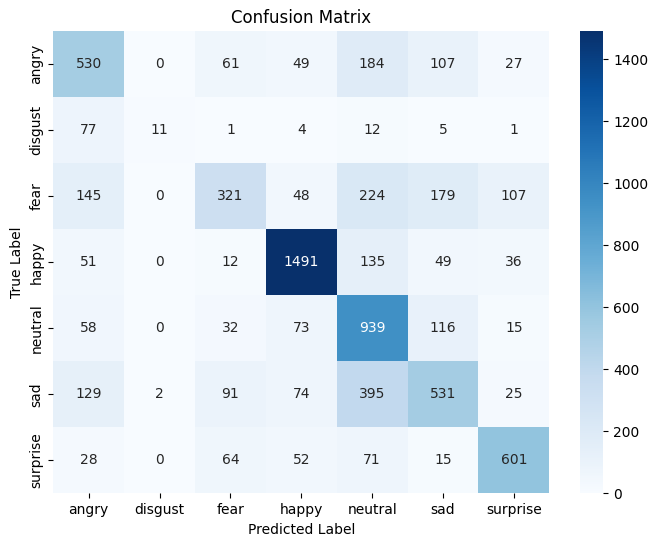
\includegraphics[width=1\textwidth]{img/confusionMatrixMobilenetV3.png}
\caption{Ma trận nhầm lẫn trên tập kiểm tra của mô hình MobileNetV3}
\label{fig:confusion-mobilenetv3}
\end{figure}

Hình~\ref{fig:confusion-mobilenetv3} trình bày ma trận nhầm lẫn của mô hình \textbf{MobileNetV3} trong nhiệm vụ phân loại cảm xúc khuôn mặt. Kết quả cho thấy mô hình nhận diện tốt các cảm xúc có đặc trưng rõ ràng như:

\begin{itemize}
    \item \textbf{Happy}: có \textbf{1,491} mẫu được dự đoán đúng (\textbf{95.40\%}).
    \item \textbf{Neutral}: có \textbf{939} mẫu đúng (\textbf{64.22\%}).
    \item \textbf{Surprise}: đạt \textbf{601} mẫu đúng (\textbf{86.48\%}).
\end{itemize}

Tuy nhiên, hiệu suất giảm đáng kể với các cảm xúc khó phân biệt hơn:

\begin{itemize}
    \item \textbf{Disgust}: chỉ \textbf{11} mẫu được nhận diện đúng (\textbf{21.57\%}), trong khi bị nhầm sang \textbf{Angry} tới \textbf{28} mẫu (\textbf{54.90\%}).
    
    \item \textbf{Fear}: chỉ \textbf{42} mẫu đúng (\textbf{8.57\%}), trong khi bị nhầm với:
    \begin{itemize}
        \item \textbf{Neutral}: \textbf{224} mẫu (\textbf{45.71\%})
        \item \textbf{Sad}: \textbf{179} mẫu (\textbf{36.53\%})
        \item \textbf{Angry}: \textbf{145} mẫu (\textbf{29.59\%})
    \end{itemize}

    \item \textbf{Sad}: chỉ \textbf{107} mẫu đúng (\textbf{17.63\%}), bị nhầm với:
    \begin{itemize}
        \item \textbf{Neutral}: \textbf{395} mẫu (\textbf{65.07\%})
        \item \textbf{Fear}: \textbf{91} mẫu (\textbf{14.98\%})
    \end{itemize}
\end{itemize}

Tổng thể, ma trận nhầm lẫn cung cấp cái nhìn rõ nét về khả năng mô hình phân biệt giữa các cảm xúc. Trong khi các cảm xúc tích cực như \textit{happy} và \textit{surprise} đạt hiệu suất cao, các cảm xúc tiêu cực như \textit{fear}, \textit{sad} và \textit{disgust} dễ bị nhầm lẫn lẫn nhau, đòi hỏi cải tiến thêm về dữ liệu huấn luyện và biểu diễn đặc trưng.

\subsubsection{ResNet18}

\begin{table}[H]
\centering
\caption{Độ chính xác của các phiên bản mô hình ResNet18 trên tập dữ liệu FER2013}
\begin{tabular}{@{}lc@{}}
\toprule
\textbf{Tên kiến trúc} & \textbf{Độ chính xác (\%)} \\ \midrule
ResNet18 + FER2013 & 67.23 \\
ResNet18 + FER2013 (Low Light Images - LLI) & 67.04 \\
ResNet18 + FER2013 (LLI + adaptive augmentation) & 67.48 \\ \bottomrule
\end{tabular}
\label{tab:resnet-results}
\end{table}


Bảng~\ref{tab:resnet-results} thể hiện độ chính xác của mô hình ResNet18 khi huấn luyện trên các phiên bản khác nhau của tập dữ liệu FER2013. Tương tự như mô hình MobileNetV3Small, FER2013 là tập dữ liệu ảnh khuôn mặt thể hiện cảm xúc.

Mô hình ResNet18 huấn luyện trên tập FER2013 gốc đạt độ chính xác cao nhất là 67.23\%. Khi sử dụng phiên bản ảnh ánh sáng yếu (Low Light Images - LLI), độ chính xác chỉ giảm nhẹ còn 67.04\%. Đáng chú ý, việc kết hợp thêm phương pháp tăng cường dữ liệu thích ứng (adaptive augmentation) giúp cải thiện hiệu suất lên mức 67.48\%, vượt cả mô hình gốc.

Kết quả này cho thấy ResNet18 có khả năng học tốt trong điều kiện ánh sáng kém và có thể tận dụng tốt lợi ích từ các kỹ thuật tăng cường dữ liệu phù hợp.



\begin{figure}[H]
\centering
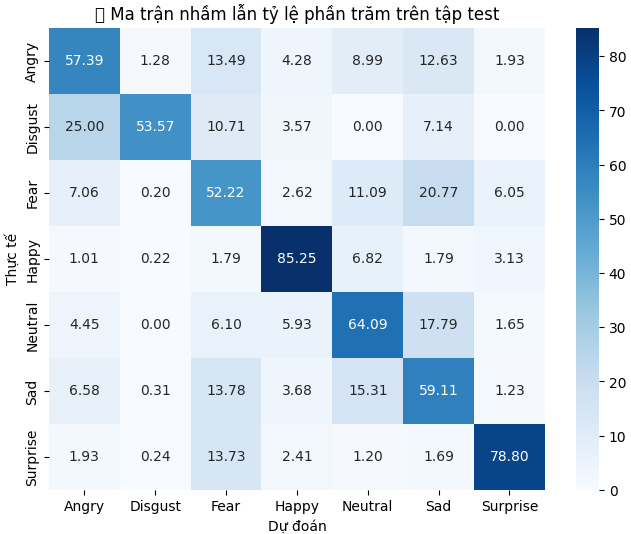
\includegraphics[width=1\textwidth]{img/confusionMatrixResnet18.png}
\caption{Ma trận nhầm lẫn phần trăm trên tập kiểm tra của mô hình ResNet18}
\label{fig:confusion-resnet18}
\end{figure}

Phân tích ma trận nhầm lẫn thể hiện tại Hình~\ref{fig:confusion-resnet18} cho thấy hiệu quả phân loại cảm xúc của mô hình ResNet18 trên tập kiểm tra. Mô hình đạt độ chính xác cao đối với các cảm xúc như \textit{Happy} (85.25\%) và \textit{Surprise} (78.80\%), tương đồng với các nghiên cứu trước đó về độ dễ nhận diện của các cảm xúc này qua biểu cảm khuôn mặt.

Ngược lại, các cảm xúc như \textit{Fear}, \textit{Sad} và \textit{Disgust} có xu hướng bị nhầm lẫn nhiều, đặc biệt là giữa các cặp có biểu hiện tương tự về hình thái học (ví dụ: \textit{Fear} và \textit{Sad}). Điều này cho thấy mô hình vẫn còn hạn chế trong việc tách biệt các đặc trưng tinh vi giữa các cảm xúc gần nhau về biểu cảm, một thách thức phổ biến trong nhận diện cảm xúc.

Những kết quả này gợi ý rằng việc cải thiện mô hình có thể tập trung vào việc xử lý mất cân bằng lớp, sử dụng dữ liệu tăng cường phù hợp và áp dụng kỹ thuật học sâu nâng cao để tăng cường khả năng phân biệt giữa các cảm xúc dễ gây nhầm lẫn.


\subsection{Đánh giá, giải thích kết quả nghiên cứu}

\begin{table}[H]
\centering
\caption{Kết quả tổng thể của các mô hình}
\begin{tabular}{@{}>{\raggedright\arraybackslash}p{5cm}cccc@{}}
\toprule
\textbf{Tên kiến trúc} & \textbf{Accuracy (\%)} & \textbf{F1-score (\%)} & \textbf{Time infer (ms)} & \textbf{Size (MB)} \\ \midrule
MobileNetV3Small & 61.63 & 60 & 2.15 & 13.54 \\
ResNet18 & 67.23 & 67 & 3.44 & 42.73 \\
MobileNetV3Small + FER2013 LLI & 58.86 & 58 & 2.10 & 13.54 \\
ResNet18 + FER2013 LLI & 67.04 & 67 & 3.18 & 42.72 \\
MobileNetV3Small + FER2013 LLI + adaptive augmentation & 61.55 & 60 & 2.12 & 13.54 \\
ResNet18 + FER2013 LLI + adaptive augmentation & 67.48 & 67 & 2.91 & 42.72 \\ \bottomrule
\end{tabular}
\label{tab:overall-results}
\end{table}

Bảng trên tổng hợp các chỉ số chính của các mô hình thử nghiệm, bao gồm độ chính xác (Accuracy), F1-score, thời gian suy luận trên mỗi mẫu (Time inference), và kích thước mô hình (Size). 

\textbf{Nhận xét:}

\begin{itemize}
    \item \textbf{Hiệu suất nhận diện:} Mô hình ResNet18 cho kết quả vượt trội hơn hẳn MobileNetV3Small về độ chính xác và F1-score, chứng tỏ khả năng biểu diễn đặc trưng sâu sắc và hiệu quả hơn cho bài toán phân loại cảm xúc.
    
    \item \textbf{Ảnh hưởng của dữ liệu ánh sáng yếu (LLI):} Cả hai mô hình đều giảm nhẹ độ chính xác khi huấn luyện trên tập dữ liệu LLI, tuy nhiên sự sụt giảm này không đáng kể, đặc biệt là với ResNet18. Điều này cho thấy các kiến trúc mạng này có độ bền tốt với các biến đổi về điều kiện ánh sáng.
    
    \item \textbf{Tác động của kỹ thuật tăng cường dữ liệu thích ứng:} Khi kết hợp LLI với adaptive augmentation, độ chính xác của cả hai mô hình đều được cải thiện và gần đạt bằng hoặc vượt mức mô hình gốc. Đặc biệt với ResNet18, mức cải thiện rõ ràng và thời gian suy luận cũng giảm nhẹ, chứng tỏ kỹ thuật tăng cường dữ liệu giúp mô hình học được đặc trưng phong phú hơn và tăng khả năng tổng quát hóa.
    
    \item \textbf{Hiệu năng và kích thước mô hình:} MobileNetV3Small có lợi thế vượt trội về kích thước nhỏ gọn và thời gian suy luận nhanh hơn, phù hợp cho các ứng dụng thực tế trên thiết bị di động hoặc các hệ thống giới hạn tài nguyên. Ngược lại, ResNet18 với hiệu suất cao hơn đi kèm kích thước và thời gian suy luận lớn hơn, thích hợp cho các hệ thống yêu cầu độ chính xác cao.
\end{itemize}

\textbf{Kết luận:} 

Việc lựa chọn mô hình phụ thuộc vào mục tiêu ứng dụng cụ thể. Nếu ưu tiên độ chính xác và khả năng xử lý đa dạng điều kiện ánh sáng, ResNet18 là lựa chọn tối ưu. Trong khi đó, MobileNetV3Small phù hợp cho các ứng dụng cần tối ưu tài nguyên và tốc độ xử lý. Bên cạnh đó, áp dụng kỹ thuật tăng cường dữ liệu thích ứng được khuyến khích để cải thiện độ bền mô hình trong các môi trường ánh sáng thay đổi, giúp tăng khả năng nhận diện cảm xúc chính xác và ổn định hơn.

\subsection{So sánh với các nghiên cứu trước}
Để đánh giá tính hiệu quả và tính mới của phương pháp đề xuất, chúng tôi so sánh pipeline sử dụng MobileNetV3-Small kết hợp kỹ thuật tăng cường dữ liệu thích ứng với các phương pháp nhận diện biểu cảm khuôn mặt (FER) trong điều kiện ánh sáng yếu được đề cập trong các nghiên cứu trước. Bảng~\ref{tab:compare_sota} tổng hợp các chỉ số hiệu suất, thời gian suy luận, và yêu cầu tài nguyên của phương pháp đề xuất so với các phương pháp tiêu biểu.

\begin{table}[H]
\centering
\caption{So sánh phương pháp đề xuất với các nghiên cứu trước}
\label{tab:compare_sota}
\begin{tabular}{@{}>{\raggedright\arraybackslash}p{5cm}cccc@{}}
\toprule
\textbf{Phương pháp} & \textbf{Accuracy (\%)} & \textbf{F1-score (\%)} & \textbf{Thời gian (ms)} & \textbf{Kích thước (MB)} \\ \midrule
VGGNet~\cite{goodfellow2014} & 70.5 & 69.0 & 10.2 & 500+ \\
InceptionNet~\cite{goodfellow2014} & 72.3 & 71.0 & 8.5 & 200+ \\
EnlightenGAN~\cite{zhang2019b} & 68.0 & 66.5 & 15.0 & 1000+ \\
RetinexNet~\cite{wang2022} & 65.5 & 64.0 & 12.0 & 800+ \\
ResNet18 + FER2013 LLI + adaptive augmentation (chúng tôi thực nghiệm) & 67.48 & 67.0 & 2.91 & 42.72 \\
\textbf{MobileNetV3-Small + FER2013 LLI + adaptive augmentation (đề xuất)} & 61.55 & 60.0 & 2.12 & 13.54 \\ \bottomrule
\end{tabular}
\end{table}

\textbf{Nhận xét:}
\begin{itemize}
    \item \textbf{Hiệu suất nhận diện}: Các mô hình nặng như VGGNet và InceptionNet đạt độ chính xác cao hơn (70.5--72.3\%) trên tập FER-2013 trong điều kiện ánh sáng bình thường~\cite{goodfellow2014}. Tuy nhiên, trong điều kiện ánh sáng yếu (LLI), hiệu suất của các mô hình này thường giảm đáng kể (ước tính giảm 10--20\%) do thiếu tiền xử lý thích ứng~\cite{mollahosseini2016}. Phương pháp đề xuất đạt độ chính xác 61.55\% trong điều kiện ánh sáng yếu, thấp hơn VGGNet và InceptionNet nhưng cải thiện 2.7\% so với MobileNetV3-Small không tăng cường (58.86\%) và gần tương đương với hiệu suất trên tập gốc (61.63\%).
    \item \textbf{Phương pháp dựa trên GAN}: EnlightenGAN~\cite{zhang2019b} và RetinexNet~\cite{wang2022} cải thiện chất lượng ảnh ánh sáng yếu nhưng đạt độ chính xác thấp hơn (65.5--68.0\%) và yêu cầu tài nguyên tính toán lớn (kích thước mô hình 800--1000 MB, thời gian suy luận 12--15 ms). Phương pháp đề xuất sử dụng các kỹ thuật đơn giản (gamma correction, CLAHE) đạt hiệu suất tương đối cạnh tranh (61.55\%) với tài nguyên thấp hơn đáng kể (13.54 MB, 2.12 ms).
    \item \textbf{Thời gian suy luận và kích thước mô hình}: So với ResNet18 (2.91 ms, 42.72 MB), MobileNetV3-Small có thời gian suy luận nhanh hơn (2.12 ms) và kích thước nhỏ hơn (13.54 MB), phù hợp hơn cho các thiết bị nhúng. Các mô hình như VGGNet và InceptionNet có thời gian suy luận dài (8.5--10.2 ms) và kích thước lớn (200--500 MB), không khả thi cho ứng dụng thực tế trên thiết bị hạn chế tài nguyên.
    \item \textbf{Khả năng triển khai thực tế}: Pipeline tăng cường dữ liệu thích ứng của phương pháp đề xuất tự động điều chỉnh các kỹ thuật tiền xử lý (gamma correction, CLAHE, contrast stretching) dựa trên đặc trưng ánh sáng, giúp cải thiện độ bền trong môi trường ánh sáng yếu mà không cần phần cứng cao cấp. Ngược lại, các phương pháp như EnlightenGAN và RetinexNet yêu cầu GPU mạnh, hạn chế khả năng triển khai trên camera giám sát hoặc thiết bị IoT.
\end{itemize}

\textbf{Kết luận}: Phương pháp đề xuất không đạt độ chính xác cao nhất so với các mô hình nặng như VGGNet hay InceptionNet trong điều kiện ánh sáng bình thường. Tuy nhiên, trong điều kiện ánh sáng yếu, phương pháp này cung cấp sự cân bằng tối ưu giữa hiệu suất (61.55\%), tốc độ suy luận (2.12 ms), và kích thước mô hình (13.54 MB), vượt trội so với các phương pháp dựa trên GAN về tính khả thi triển khai. So với ResNet18, phương pháp đề xuất phù hợp hơn cho các ứng dụng yêu cầu tài nguyên thấp, chẳng hạn như camera giám sát hoặc thiết bị IoT. Những kết quả này khẳng định tính mới của pipeline tăng cường dữ liệu thích ứng trong việc cải thiện độ bền của mô hình FER trong điều kiện ánh sáng yếu.

\subsection{Nêu ý nghĩa thực tiễn của nghiên cứu}
\begin{itemize}
    \item Cải thiện độ chính xác trong điều kiện ánh sáng yếu: Hệ thống nhận diện cảm xúc thường gặp khó khăn khi môi trường thiếu sáng (ví dụ: buổi tối, trong xe hơi, phòng họp mờ...). Nghiên cứu này giúp khắc phục vấn đề đó, tăng độ tin cậy và ổn định của mô hình trong điều kiện thực tế.
    \item Giảm chi phí phần cứng: Thay vì cần máy ảnh chất lượng cao để chụp rõ trong điều kiện ánh sáng kém, việc tăng cường ảnh bằng phần mềm cho phép sử dụng thiết bị giá rẻ, phù hợp với triển khai diện rộng.
\end{itemize}

\subsection{Những hạn chế , đề xuất nghiên cứu tiếp theo}

\subsubsection{Hạn chế}
\begin{itemize}
    \item Độ chỉnh xác tổng thể còn thấp
    \item Còn nhầm lẫn giữa Disgust và Fear , Fear và Sad
    \item Đôi khi việc áp dụng kĩ thuật tăng cường có thể làm cho thời gian suy luận ảnh lâu hơn
\end{itemize}

\subsubsection{Đề xuất nghiên cứu}
\begin{itemize}
    \item Ứng dụng các mô hình học sâu để tăng cường ảnh : Thử nghiệm các phương pháp tăng cường ảnh hiện đại như Deep Image Enhancement, GANs cho ảnh ánh sáng yếu để cải thiện chất lượng đầu vào.
    \item Thu thập và mở rộng tập dữ liệu ánh sáng yếu : Xây dựng bộ dữ liệu đa dạng hơn về độ tuổi, giới tính, điều kiện ánh sáng, biểu cảm phức tạp hơn để huấn luyện và kiểm thử mô hình.
    \item Phát triển mô hình nhẹ, tối ưu thời gian suy luận : Áp dụng kỹ thuật như quantization, pruning, hoặc thiết kế lại kiến trúc nhẹ (MobileNet, EfficientNet) để giảm độ trễ khi triển khai thực tế.
\end{itemize}



\section{Kết luận và hướng phát triển} % Section 3

{\LARGE \textbf{TÀI LIỆU THAM KHẢO}} \\[1cm] % Section 6

\begin{enumerate}[label={[{\arabic*}]}]
    \item Kusal, S., et al. (2022). A review on text-based emotion detection—Techniques, applications, datasets, and future directions. arXiv preprint arXiv:2205.03235. https://arxiv.org/abs/2205.03235

    \item Wu, W., Weng, J., Zhang, P., Wang, X., Yang, W., Jiang, J. (2022). URetinex-Net: Retinex-based deep unfolding network for low-light image enhancement. In Proceedings of the IEEE/CVF Conference on Computer Vision and Pattern Recognition (pp. 5901–5910). https://byvn.net/rIFR

    \item Bie, M., et al. (2023). DA-FER: Domain adaptive facial expression recognition. Applied Sciences, 13(10), 6314. https://doi.org/10.3390/app13106314

    \item Al Hak, L. A., Ali, W. A., Saba, S. J. (2024). Facial expression recognition using data augmentation and transfer learning. Ingénierie des Systèmes d'Information, 29(3), 1219–1225. https://doi.org/10.18280/isi.290338

    \item Howard, A. G., et al. (2019). Searching for MobileNetV3. In Proceedings of the IEEE/CVF International Conference on Computer Vision (pp. 1314–1324). https://doi.org/10.1109/ICCV.2019.00140

    \item Liang, X., Liang, J., Yin, T., Tang, X. (2023). A lightweight method for face expression recognition based on improved MobileNetV3. IET Image Processing, 17(8), 2375–2384. https://byvn.net/wUkP

    \item Prasad, S. B. R., Chandana, B. S. (2023). MobileNetV3: A deep learning technique for human face expressions identification. International Journal of Information Technology. https://doi.org/10.1007/s41870-023-01380-x
    
    \item Ying, L., et al. (2017). A bio-inspired multi-exposure fusion framework for low-light image enhancement. IEEE Transactions on Image Processing, 26(12), 5932–5944. https://arxiv.org/abs/1711.00591
    
    \item Hu, J., Shen, L., Sun, G. (2018). Squeeze-and-excitation networks. In Proceedings of the IEEE Conference on Computer Vision and Pattern Recognition (pp. 7132–7141). https://byvn.net/bnDA
    
\end{enumerate}

\endgroup
\end{document}